%
% TERMINADA, PORFAVOR REVISAR
%
En un departamento de control de calidad se inspeccionan las unidades terminadas que provienen de una l\'inea de ensamble.
Se piensa que la proporci\'on de unidades defectuosas es 0.09.
% Binomial Negativa
% P = 0.09
\begin{itemize}
	\item ?`Cu\'al es la probabilidad de que la d\'ecima unidad inspeccionada es la tercera defectuosa detectada?\\
		Para que el tercer exito este dentro de los 10 intentos, se considera 7 fracasos.\\
		$P(X=7)\ =\ 0.01356188$\\ % dnbinom(7,3,0.09)
	\item ?`Cu\'al es la probabilidad de que la vig\'esima unidad inspeccionada es la quinta defectuosa detectada?\\
		Para que el quinto exito este dentro de los 20 intentos, se consideran 15 fracasos.\\
		$P(X=15)\ =\ 0.005561823$\\% dnbinom(15,5,0.09)
	\item ?`En qu\'e numero de inspecci\'on se espera encontrar 4 unidades defectuosas? ?`Cu\'al es su varianza?\\
		La cantidad de fracasos esperados es:
		$$ \bar{x}\ =\ \frac{4\cdot(1-0.09)}{0.09}\ =\ 40.444 $$
		% $media(x)\ =\ \frac{4(1-0.09)}{0.09}$\\
		Y su varianza es de:
		 $$Varianza\ =\ Var(x)\ =\ \frac{4(1-0.09)}{0.09^2}\ =\ 449.3827 $$
		% $Varianza\ =\ Var(x)\ =\ \frac{4(1-0.09)}{0.09^2}$\\
	\item Realice gr\'aficos de la funci\'on de densidad de probabilidad y de la funci\'on de distribuci\'on.\\
	Funci\'on de densidad de probabilidad con 4 numeros de fallas:\\
  	  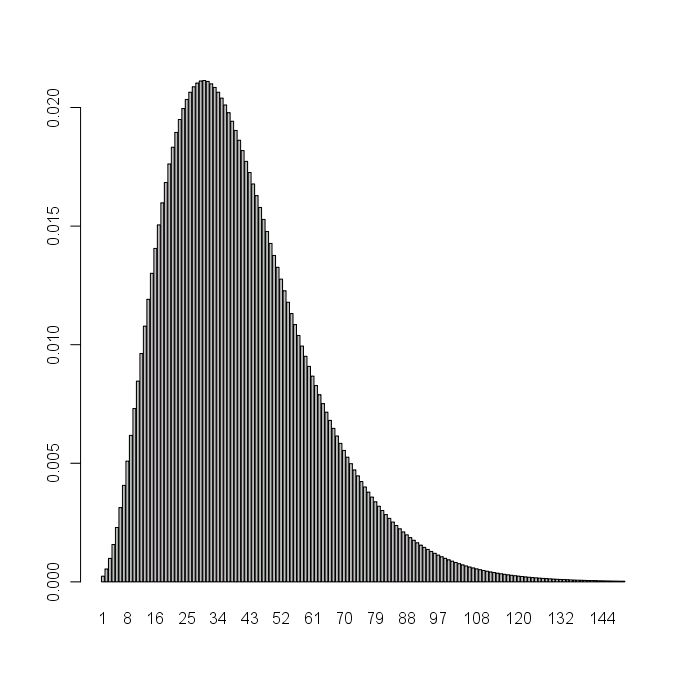
\includegraphics[width=3.3in,height=3.3in]{images/1_3-dnbinom.png}\\
	Funci\'on de distribucion con 4 numeros de fallas:\\
  	  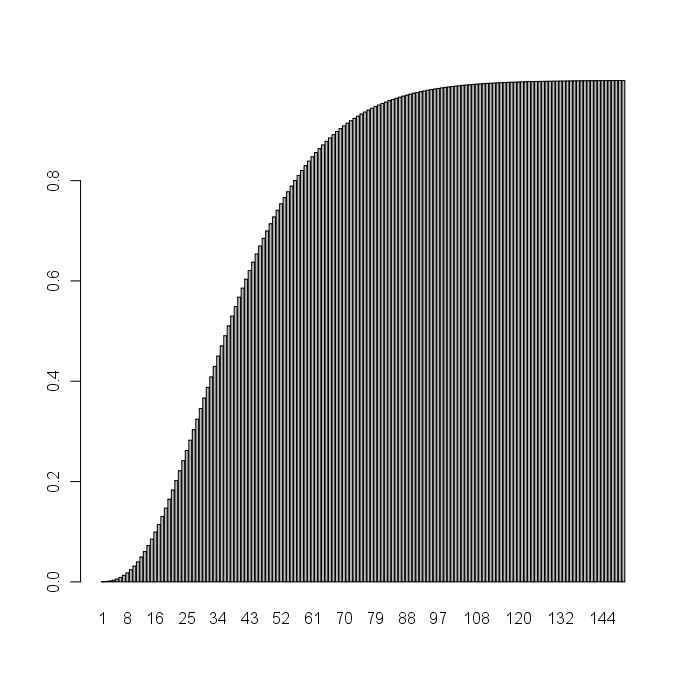
\includegraphics[width=3.3in,height=3.3in]{images/1_3-pnbinom.png}
		%x<-seq(1,40)
		%k<-seq(1,40) No se como asignar una cantidad de fallas para el grafico...se me ocurrio una secuencia nomas...
		% barplot(dnbinom(x,k,0.09),names.arg=x)
		% barplot(pnbinom(x,k,0.09),names.arg=x)	
	\item Var\'ie el o los valores de los par\'ametros de la distribuci\'on y comente lo observado en los gr\'aficos de la funci\'on de densidad y de distribuci\'on. (2 casos)\\\\
	Caso 1: Variando el numero de fallas a 16.\\
	Funci\'on de densidad de probabilidad con k =16\\
  	  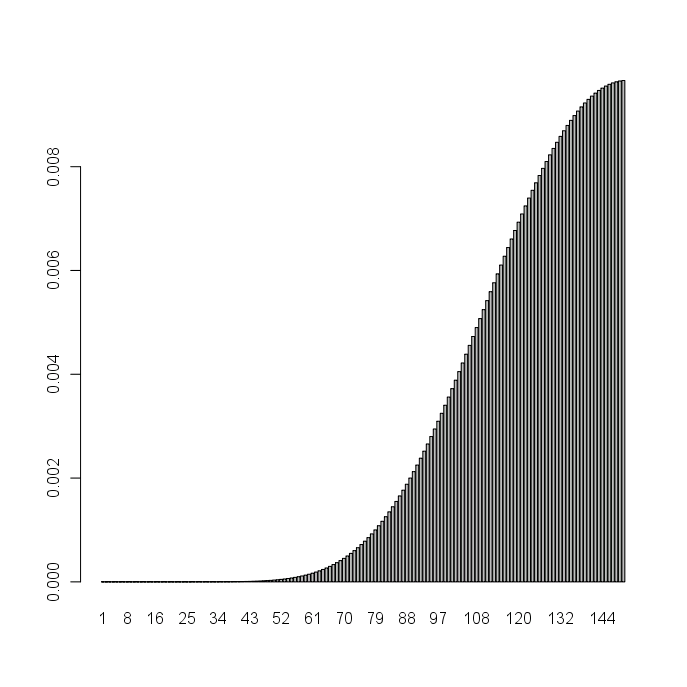
\includegraphics[width=3.3in,height=3.3in]{images/1_3-dnbinom16.png}\\
	Funci\'on de distribucion con k = 16 \\
  	  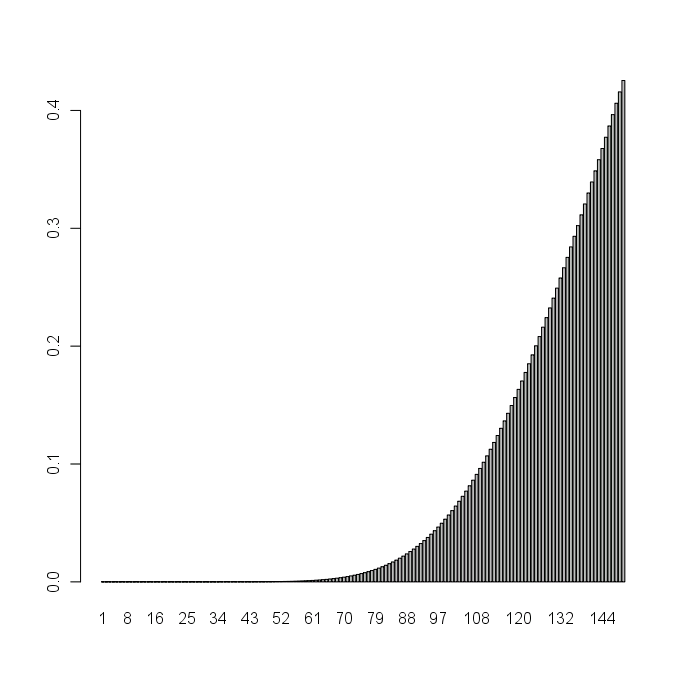
\includegraphics[width=3.3in,height=3.3in]{images/1_3-pnbinom16.png}\\
	Caso 2: Variando la probabilidad de obtener una falla a 0.18:\\
	Funci\'on de densidad de probabilidad con p = 0.18 \\
  	  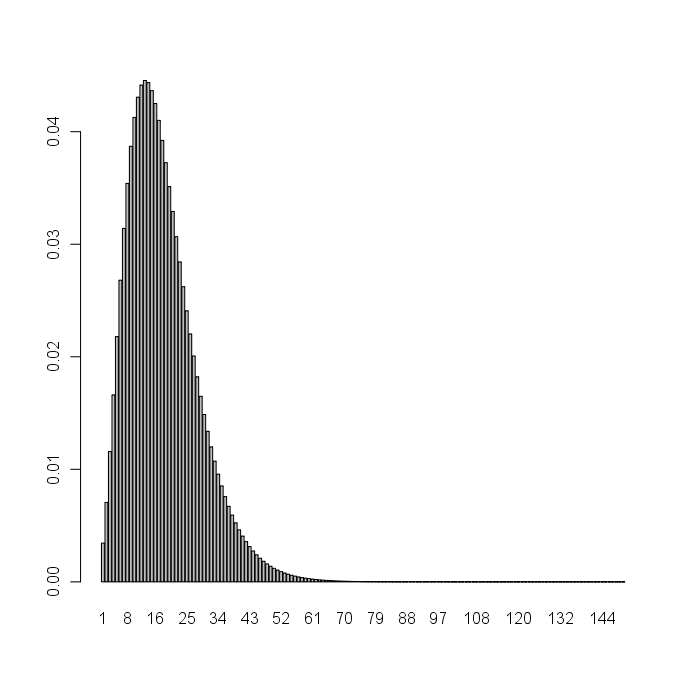
\includegraphics[width=3.3in,height=3.3in]{images/1_3-dnbinom018.png}\\
	Funci\'on de distribuci\'on con p = 0.18\\
  	  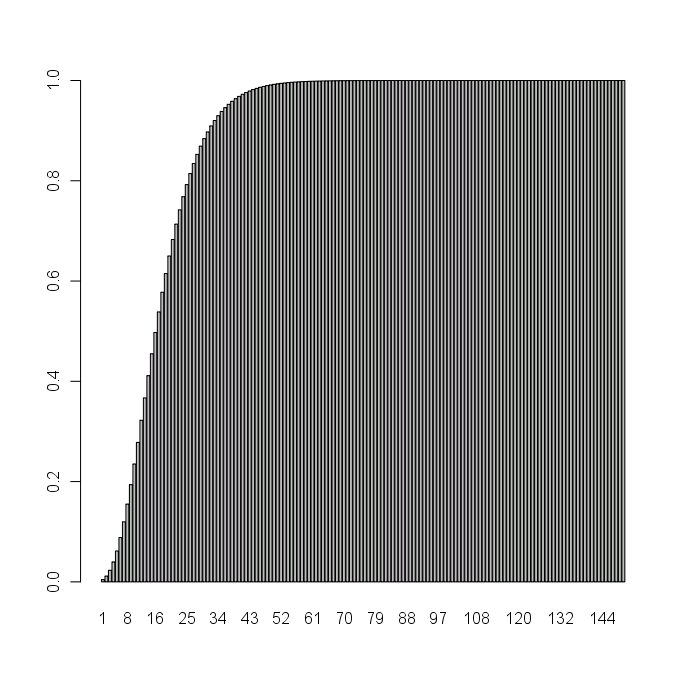
\includegraphics[width=3.3in,height=3.3in]{images/1_3-pnbinom018.png}\\

	Claramente podemos observar como al aumentar el numero de fallas esperadas, la probabilidad crece mucho mas lentamente, expandiendose y corriendose la forma del gr\'afico hacia la derecha, y al aumentar la probabilidad de obtener fallas, el gr\'afico tiene a comprimirse y correrse mas hacia la izquierda, aumentando considerablemente la pendiente de la probabilidad acumulada.
\end{itemize}
